% Appendix C: Spatial Analysis Details

\section*{Appendix C: Spatial Analysis Details}
\label{appendix:spatial}

The empirical models predict accuracy from \emph{mean} reachability, but reachability varies spatially within each network---boundary areas have lower reachability than network centres. This raises an important question: does sampling accuracy hold uniformly across the network, or do low-reachability areas show systematically worse accuracy?

We investigate this by analysing accuracy separately for nodes grouped by local reachability quartile. For each city (London, Madrid, Phoenix) and distance threshold (500m, 1000m, 2000m), we compute ground truth centrality, then compare against sampled estimates ($p = 0.30$, averaged over 3 runs). Table~\ref{tab:spatial_reachability} summarises accuracy by reachability quartile.

% Auto-generated table (from benchmark_regional.py)
\InputIfFileExists{tables/spatial_reachability.tex}{}{%
  \textbf{[Table not yet generated. Run: python benchmark\_regional.py]}%
}

\subsection*{Non-Monotonic Pattern for Harmonic Closeness}

A surprising finding emerges: harmonic closeness accuracy does not increase monotonically with reachability. Instead, we observe a U-shaped pattern where Q1 (lowest reachability) and Q4 (highest reachability) both show higher accuracy than the middle quartiles Q2 and Q3.

Figure~\ref{fig:spatial_quartiles} shows this pattern is consistent across all three cities. Boundary nodes (Q1) achieve $\rhospH \approx{}$\spatialQlowH{} despite having the lowest effective sample size, while transitional zones (Q2--Q3) show reduced accuracy with $\rhospH$ dropping to \spatialQmidHrange{}. Dense core nodes (Q4) recover to $\rhospH \approx{}$\spatialQhighH{}.

% Auto-generated figure (from benchmark_regional.py)
\begin{figure}[htbp]
    \centering
    \IfFileExists{figures/spatial_reachability_accuracy.pdf}{%
        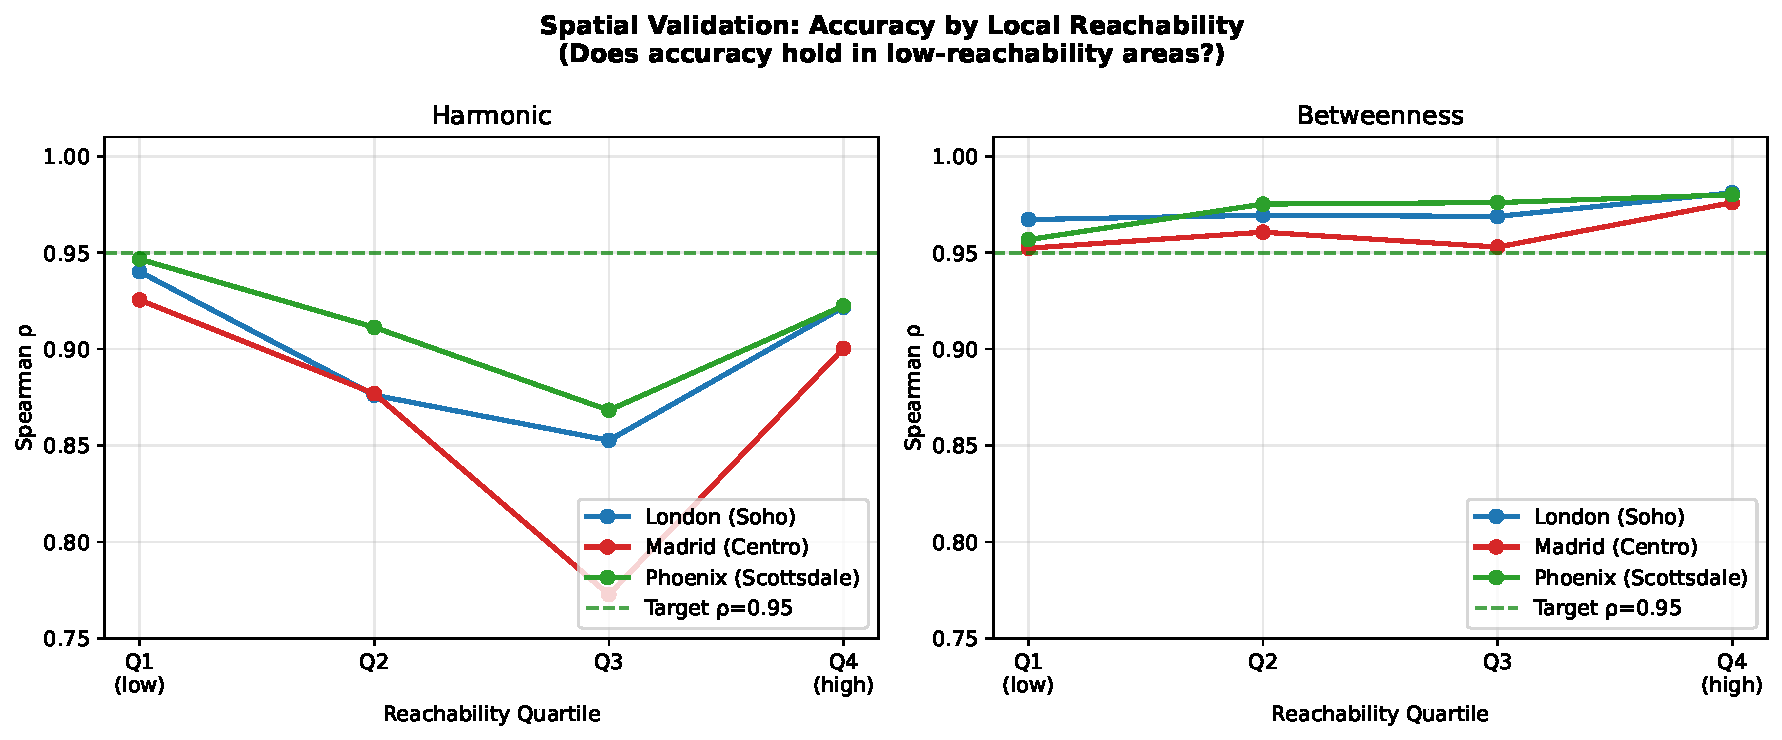
\includegraphics[width=\textwidth]{figures/spatial_reachability_accuracy.pdf}%
    }{%
        \fbox{\parbox{0.8\textwidth}{\centering\vspace{2cm}[Figure not yet generated.\\Run: python benchmark\_regional.py]\vspace{2cm}}}%
    }
    \caption{Accuracy by local reachability quartile. Left: harmonic closeness shows a non-monotonic U-shaped pattern across all three cities. Right: betweenness shows the expected monotonic increase with reachability.}
    \label{fig:spatial_quartiles}
\end{figure}

Betweenness centrality, in contrast, shows the expected monotonic pattern: accuracy increases consistently from Q1 to Q4, and remains above the $\rhosp = 0.95$ target across all quartiles.

\subsection*{Spatial Clustering of Residuals}

To assess whether errors are spatially structured, we compute Moran's I \citep{Moran1950} for the residuals (relative error between sampled and true values). Table~\ref{tab:morans_i} summarises the spatial autocorrelation.

\begin{table}[htbp]
\centering
\caption{Moran's I spatial autocorrelation of sampling residuals. Higher values indicate stronger spatial clustering of errors.}
\label{tab:morans_i}
\InputIfFileExists{tables/morans_i.tex}{}{%
  \textbf{[Table not yet generated. Run: python benchmark\_regional.py]}%
}
\end{table}

Harmonic closeness residuals show substantial spatial clustering (Table~\ref{tab:morans_i}), while betweenness residuals are more dispersed. Figure~\ref{fig:residual_maps} visualises the spatial distribution of residuals.

\begin{figure}[htbp]
    \centering
    \includegraphics[width=\textwidth]{figures/spatial_residuals_map.png}
    \caption{Spatial distribution of estimation residuals. Harmonic closeness residuals show coherent spatial clusters, particularly at network boundaries. Betweenness residuals show a more dispersed pattern.}
    \label{fig:residual_maps}
\end{figure}

\subsection*{Interpretation}

The non-monotonic pattern for harmonic closeness can be understood through network topology. Boundary nodes (Q1) have truncated catchments extending predominantly in one direction, making the distance-weighted sum more predictable from a sample. Transitional nodes (Q2--Q3) sit at the interface between dense and sparse areas with complex, asymmetric catchment structures and multiple competing paths, making sampled estimates more variable. Dense core nodes (Q4) have high connectivity with many redundant paths, so sampling any subset captures the essential structure. Betweenness does not show this pattern because it measures path \emph{flow} rather than \emph{proximity}---the flow structure depends on global network topology rather than local catchment shape, so accuracy scales more directly with effective sample size.

\subsection*{Implications for Practice}

These findings indicate that betweenness accuracy is well-predicted by effective sample size alone, while harmonic closeness exhibits additional topology-dependent variance. The accuracy dip in transitional zones is most pronounced at short distances (500m) and diminishes at longer distances. Section~\ref{sec:discussion} provides guidance on adjusting target accuracy for these cases.
